\documentclass{article}
\usepackage[utf8]{inputenc}
\usepackage[margin=2cm]{geometry}

\usepackage{graphicx}
\usepackage{enumitem}

% custom header/footer
\usepackage{fancyhdr}
\pagestyle{fancy}
\renewcommand{\headrulewidth}{0pt}
\fancyhf{}
\rfoot{\textsf{\thepage}}
\lfoot{\textsf{Suzie Brown}}

%annotations
\usepackage{color}
\usepackage{xspace}
\newcommand{\seb}[1]{\xspace\textcolor{red}{#1}\xspace}

% bibliography
\usepackage[round, sort&compress]{natbib}
\usepackage{har2nat}
\bibliographystyle{agsm}

% maths
\usepackage{amsmath}
\usepackage{amssymb}
\usepackage{amsthm}
\newtheorem{thm}{Theorem}
\newtheorem{lemma}{Lemma}
\newcommand{\PR}{\mathbb{P}}
\newcommand{\E}{\mathbb{E}}
\newcommand{\V}{\operatorname{Var}}
\newcommand{\I}[1]{\mathbb{I}_{\{#1\}}}
\newcommand{\Mn}{\operatorname{Multinomial}}

\title{Non-triviality condition (shortened version)}
\author{Suzie Brown}

\begin{document}
\maketitle
\thispagestyle{fancy}

The following theorem will be used in each section. It is a version of the second Borel--Cantelli lemma, which can be found for instance in [Durrett, Theorem 4.3.4 - make citation].
\begin{thm}
Let$ (\mathcal{F}_n)_{n\geq 0}$ be a filtration with $\mathcal{F}_0 = \{\emptyset, \Omega\}$. Let $(B_n)_{n\geq 0}$ be a sequence of events such that $B_n \in \mathcal{F}_n$ for all $n$.
Then the events $\{ B_n \, i.o. \}$ and $\{ \sum_{n=1}^\infty \PR[B_n \mid \mathcal{F}_{n-1} ] =\infty \}$ are almost surely equal.
\end{thm}


\section*{Multinomial resampling}

\begin{lemma}\label{lem:neutral_cN_LB}
For all $N\geq 2$, for all $t$,
\begin{equation*}
\PR \left[c_N(t) > \frac{2}{N^2} \middle| \mathbf{w}=\left( \frac{1}{N}, \dots, \frac{1}{N} \right) \right] 
= 1- \frac{N!}{N^N}.
\end{equation*}
\end{lemma}

\begin{proof}
Fix arbitrary $t$ and $N\geq 2$. Since $2/(N)_2 > 2/(N^2)$ is the smallest possible non-zero value for $c_N(t)$,
\begin{align*}
\PR \left[c_N(t) > \frac{2}{N^2} \mid \mathbf{w}=(1/N, \dots, 1/N) \right]
&= 1- \PR[c_N(t) = 0  \mid \mathbf{w}=(1/N, \dots, 1/N)] \\
&= 1- \PR[\nu_t^{(1:N)} = (1,\dots, 1) \mid \mathbf{w}=(1/N, \dots, 1/N)].
\end{align*}
Conditional on the weights, $\nu_t^{(1:N)} \sim \Mn(N, (1/N, \dots, 1/N))$, so the probability of interest is
\begin{equation*}
\PR[\nu_t^{(1:N)} = (1,\dots, 1) \mid \mathbf{w}=(1/N, \dots, 1/N)] =
N! \prod_{i=1}^N \frac{1}{N}
= \frac{N!}{N^N}.
\end{equation*}
\end{proof}


\begin{lemma}\label{thm:nontrivial_mn_optimalw}
In the neutral case (i.e.\ when all weights are equal at every time step) with multinomial resampling, there exists $N_0$ such that for all $N>N_0$, for all finite $t$, $\PR[\tau_N(t) = \infty] =0$.
\end{lemma}

\begin{proof}
Let us rewrite the event of interest in a different way.
\begin{align*}
\PR[\tau_N(t) = \infty] =0 &\Leftrightarrow \PR[\tau_N(t) < \infty] =1 \\
&\Leftrightarrow \PR\left[ \min \left\{s>1 : \sum_{r=1}^s c_N(r) >t \right\} < \infty \right] =1 \\
&\Leftrightarrow \PR\left[ \exists s<\infty : \sum_{r=1}^s c_N(r) >t \right] =1
\end{align*}
It is sufficient to show that, almost surely for all $N>N_0$, $c_N(r)$ is bounded away from zero infinitely often in $r$.
We consider the sequence of events 
$E_r := \{ c_N(r) > 2/N^2 \}$ for $r \in \mathbb{N}$.
In the neutral case, the resampled family sizes at each generation are independent, hence the events $E_r$ are independent. 
By the second Borel-Cantelli lemma, $E_r$ occurs infinitely often if $\sum_{r=1}^\infty \PR(E_r) = \infty$. 
An expression for $\PR(E_r)$ is given in Lemma \ref{lem:neutral_cN_LB}. 
For any fixed $N\geq 2$, the probability is strictly positive and constant in $r$, so the Borel-Cantelli condition is satisfied, thus we conclude that $E_r$ occurs infinitely often.
Hence, taking $N_0=1$, we have that $\PR[\tau_N(t) = \infty] =0$ for all $N>N_0$ and all finite $t$, as required.
\end{proof}


\begin{lemma}\label{lem:mn_optimal_w}
For all $N\geq 2$, for all $t$, for any weight vector $(w_1, \dots, w_N) \in \mathcal{S}_{N-1}$,
\begin{equation*}
\PR \left[c_N(t) > \frac{2}{N^2} \middle| \mathbf{w}=(w_1, \dots, w_N) \right]
\geq \PR \left[c_N(t) > \frac{2}{N^2} \middle| \mathbf{w}=\left( \frac{1}{N}, \dots, \frac{1}{N} \right) \right] .
\end{equation*}
That is, the probability of having at least one merger is minimised by the vector of equal weights.
\end{lemma}

\begin{proof}
Fix arbitrary $t$ and $N\geq 2$. Recall that
\begin{equation}\label{eq:mn_nomerger_prob}
1-\PR \left[c_N(t) > \frac{2}{N^2} \mid \mathbf{w}=(w_1, \dots, w_N) \right]
= N! \prod_{i=1}^N w_i .
\end{equation}
We will show that the global maximum of this function on the simplex $\mathcal{S}_{N-1}$ is attained at $\mathbf{w}=(1/N,\dots,1/N)$.
This weight vector will therefore minimise the probability of the complementary event, implying the desired result.

First, since we are working on the simplex, we encode the constraint $\sum w_j =1$ by rewriting the function to optimise as
\begin{equation*}
f(\mathbf{w}) :=
\prod_{i=1}^N w_i
= \left(1- \sum_{j=1}^{N-1} w_j \right)\prod_{i=1}^{N-1} w_i 
\end{equation*}
where we have also dropped the constant positive factor $N!$. Note that this objective function is non-negative and obtains its minimal value zero whenever one or more of the weights is equal to zero; since we are looking for a maximum we can assume that $w_i >0$ for all $i$.
Now, for every $k \in \{1,\dots,N-1\}$, we solve
\begin{equation*}
\frac{\partial f(\mathbf{w})}{\partial w_k}
= \left(1- w_k - \sum_{j=1}^{N-1} w_j \right)\prod_{i\neq k}^{N-1} w_i 
=0 .
\end{equation*}
The product over $i \neq k$ is constant and positive for each $k$, so this amounts to solving
\begin{equation*}
w_k = 1- \sum_{j=1}^{N-1} w_j = w_N
\end{equation*}
for all $k$.
The unique solution is
$w_1 = w_2= \dots =  w_N = 1/N$.

To verify that the critical point is a maximum, we evaluate the Hessian $H$:
\begin{align*}
H_{kl}(\mathbf{w})
&= \begin{cases}
-2 \prod_{i\neq k}^{N-1} w_i & k=l \\
\left( 1 - w_k - w_l - \sum_{j=1}^{N-1} w_j \right)\prod_{i\neq k,l}^{N-1}w_i & k\neq l
\end{cases} \\
H_{kl}(1/N, \dots, 1/N)&= \begin{cases}
-2 \left(\frac{1}{N}\right)^{N-2} & k=l \\
- \left(\frac{1}{N}\right)^{N-2} & k\neq l
\end{cases}
\end{align*}
and show that $H$ is negative definite at $(1/N, \dots, 1/N)$: for any $\mathbf{x} \in \mathbb{R}^{N-1} \setminus \{\mathbf{0}\}$,
\begin{align*}
\mathbf{x}^T H\left(\frac{1}{N}, \dots, \frac{1}{N}\right) \mathbf{x} &= \sum_{k=1}^{N-1} \left[ -2\left(\frac{1}{N}\right)^{N-2} x_k^2
- \sum_{l\neq k}^{N-1} \left(\frac{1}{N}\right)^{N-2} x_k x_l \right] 
= \left(\frac{1}{N}\right)^{N-2} \left[ -\sum_{k=1}^{N-1} 2x_k^2 - \sum_{k=1}^{N-1} \sum_{l\neq k}^{N-1} x_k x_l \right] \\
&= \left(\frac{1}{N}\right)^{N-2} \left[ -\sum_{k=1}^{N-1} x_k^2 - \sum_{k=1}^{N-1} \sum_{l=1}^{N-1} x_k x_l \right]
= \left(\frac{1}{N}\right)^{N-2} \left[ - \sum_{k=1}^{N-1} x_k^2 - \left(\sum_{k=1}^{N-1} x_k \right)^2 \right]
< 0 .
\end{align*}
\end{proof}

\begin{thm}
With multinomial resampling, conditional on any sequence of weight vectors $\mathbf{w}_r^{(1:N)} \in \mathcal{S}_{N-1}; r\in\mathbb{N}$, there exists $N_0$ such that for all $N>N_0$, for all finite $t$, $\PR[\tau_N(t) = \infty] =0$.
\end{thm}

\begin{proof}
As in Lemma \ref{thm:nontrivial_mn_optimalw}, denote the sequence of events 
$E_r := \{ c_N(r) > 2/N^2 \}$ for $r \in \mathbb{N}$.
We know from Lemma \ref{thm:nontrivial_mn_optimalw} that, in the neutral case, $E_r$ occurs infinitely often. Lemma \ref{lem:mn_optimal_w} tells us that 
$\PR[E_r \mid \mathbf{w}=(w_1, \dots, w_N)] \geq \PR[E_r \mid \mathbf{w}=(1/N, \dots, 1/N)]$
for all $r$. 
Therefore, by a coupling argument, we conclude that $E_r$ occurs infinitely often in the non-neutral case as well.
\end{proof}


\section*{Conditional SMC with multinomial resampling}

Define $\mathbf{w}^* := \frac{1}{N-1} \left[ (1,\dots,1) - \mathbf{e}_{i^*} \right]$, where $i^*$ is the immortal index at generation $t$, and $\mathbf{e}_i$ denotes the $i^{th}$ canonical basis vector.
 
\begin{lemma}\label{lem:csmc_cN_LB}
For all $N\geq 2$, for all $t$,
\begin{equation*}
\PR \left[c_N(t) > \frac{2}{N^2} \middle| \mathcal{H}_t, \mathbf{w}_t=\mathbf{w}^*  \right] 
= 1- (\varepsilon(N-1))^{1-N} \prod_{i\neq i^*}^N h(X_{t-1}^{(i)}) .
\end{equation*}
\end{lemma}

\begin{proof}
Under $\mathbf{w}^*$, the immortal parent has zero weight and is therefore assigned exactly one offspring (the immortal particle). The remaining $N-1$ offspring are assigned to the remaining $N-1$ parents according to a Multinomial distribution with equal weights. We therefore have
\begin{align*}
\PR \left[c_N(t) \leq \frac{2}{N^2} \mid \mathcal{H}_t \right]
&=\frac{1}{(N-1)!} \sum_{\mathbf{a}_t : \nu_t^{(i)}=1 \forall i} \PR[\mathbf{a}_t \mid \mathcal{H}_t] \\
&=\frac{1}{(N-1)!} \sum_{\mathbf{a}_t: \nu_t^{(i)}=1 \forall i} \prod_{i \neq i^*}^N w_t^{(i)} q_{t-1}(X_t^{(a_t^{(i)}}, X_{t-1}^{(i)}) \\
&\leq \frac{1}{(N-1)!} \sum_{\mathbf{a}_t: \nu_t^{(i)}=1 \forall i} \prod_{i \neq i^*}^N w_t^{(i)} \varepsilon^{-1} h(X_{t-1}^{(i)}) \\
&= \prod_{i \neq i^*}^N w_t^{(i)} \varepsilon^{-1} h(X_{t-1}^{(i)}) \\
&= \varepsilon^{1-N} \left( \prod_{j \neq i^*}^N w_t^{(j)} \right) \left( \prod_{i \neq i^*}^N h(X_{t-1}^{(i)}) \right) \\
&\propto \prod_{j \neq i^*}^N w_t^{(j)} =: f(\mathbf{w}_t) .
\end{align*}
Evaluated at $\mathbf{w}^*$, we have 
\begin{equation*}
\PR \left[c_N(t) > \frac{2}{N^2} \middle| \mathcal{H}_t, \mathbf{w}_t=\mathbf{w}^*  \right] 
= 1- \varepsilon^{1-N} \left( \prod_{j \neq i^*}^N \frac{1}{N-1} \right) \left( \prod_{i \neq i^*}^N h(X_{t-1}^{(i)}) \right)
= 1- (\varepsilon(N-1))^{1-N} \prod_{i\neq i^*}^N h(X_{t-1}^{(i)})
\end{equation*}
as required.
\end{proof} 

 
\begin{lemma}\label{thm:nontrivial_csmc_optimalw}
In conditional SMC with multinomial resampling, in the optimal case where the weight vector is equal to $\mathbf{w}^*$ at every time step, there exists $N_0$ such that for all $N>N_0$, for all finite $t$, $\PR[\tau_N(t) = \infty] =0$.
\end{lemma}

\begin{proof}
The proof is exactly the same as for Lemma \ref{thm:nontrivial_mn_optimalw}; Lemma \ref{lem:csmc_cN_LB} provides the expression for $P(E_r)$ which is strictly positive and constant in $r$.
\end{proof}


\begin{lemma}\label{lem:csmc_optimal_w}
For all $N\geq 2$, for all $t$, for any weight vector $(w_1, \dots, w_N) \in \mathcal{S}_{N-1}$,
\begin{equation*}
\PR \left[c_N(t) > \frac{2}{N^2} \middle| \mathcal{H}_t \right]
\geq \PR \left[c_N(t) > \frac{2}{N^2} \middle| \mathcal{H}_t, \mathbf{w}_t = \mathbf{w}^* \right].
\end{equation*}
\end{lemma}

\begin{proof}
In the proof of Lemma [4] we found an expression for the probability of interest, $\PR[c_N(t) \leq 2/N^2 \mid \mathcal{H}_t]$.
To see that $\mathbf{w}^*$ is the ``worst case'' weight vector (i.e\ maximising that probability), consider the optimisation of
\begin{equation*}
f(\mathbf{w}) :=
\prod_{\substack{i=1\\ i\neq i^*}}^N w_i
= \left(1- \sum_{j=1}^{N-1} w_j \right)\prod_{\substack{i=1\\ i\neq i^*}}^{N-1} w_i 
\propto \PR \left[c_N(t) \leq \frac{2}{N^2} \mid \mathcal{H}_t, \mathbf{w}_t = \mathbf{w} \right]
\end{equation*}
over $\mathbf{w} \in \mathcal{S}_{N-1}$.
This objective function is non-negative and obtains its minimal value zero whenever one or more of the non-immortal weights is equal to zero; since we are looking for a maximum we can assume that $w_i >0$ for all $i \neq i^*$.
Now, for every $k \in \{1,\dots,N-1\}\setminus \{i^*\}$, we solve
\begin{equation*}
\frac{\partial f(\mathbf{w})}{\partial w_k}
= \left(1- w_k - \sum_{j=1}^{N-1} w_j \right)\prod_{\substack{i=1\\ i\neq k,i^*}}^{N-1} w_i 
=0 .
\end{equation*}
The product is constant and positive for each $k$, so this amounts to solving
\begin{equation*}
w_k = 1- \sum_{\substack{j=1\\ j\neq i^*}}^{N-1} w_j = w_N
\end{equation*}
simultaneously for all $k \in \{1,\dots,N-1\}\setminus \{i^*\}$.
The locus of solutions is the ridge
$\mathbf{w}_a = \{(1, \dots,1) +a \mathbf{e}_{i^*} \} /(N+a)$ for some constant $a \in [-1,\infty)$. (See Figure \ref{fig:CSMC_ternaryplot} for an illustration in the case N=3.)
It can be shown that the Hessian in indices $\{1,\dots,N\}\setminus \{i^*\}$ is negative definite.
\seb{The Hessian in the non-immortal indices comes out exactly as in the standard multinomial case; a proof analogous to that one could easily be included.}
On this ridge the objective function takes values $f(\mathbf{w}_a) = (N+a)^{1-N}$.
Further optimising over $a$, the unique maximum is at $a=-1$, thus $\mathbf{w}^* = \{(1,\dots,1) - \mathbf{e}_{i^*}\} /(N-1)$.
This weight vector thus minimises the probability of the complementary event, and we conclude the result.
\end{proof}

\begin{figure}
\centering
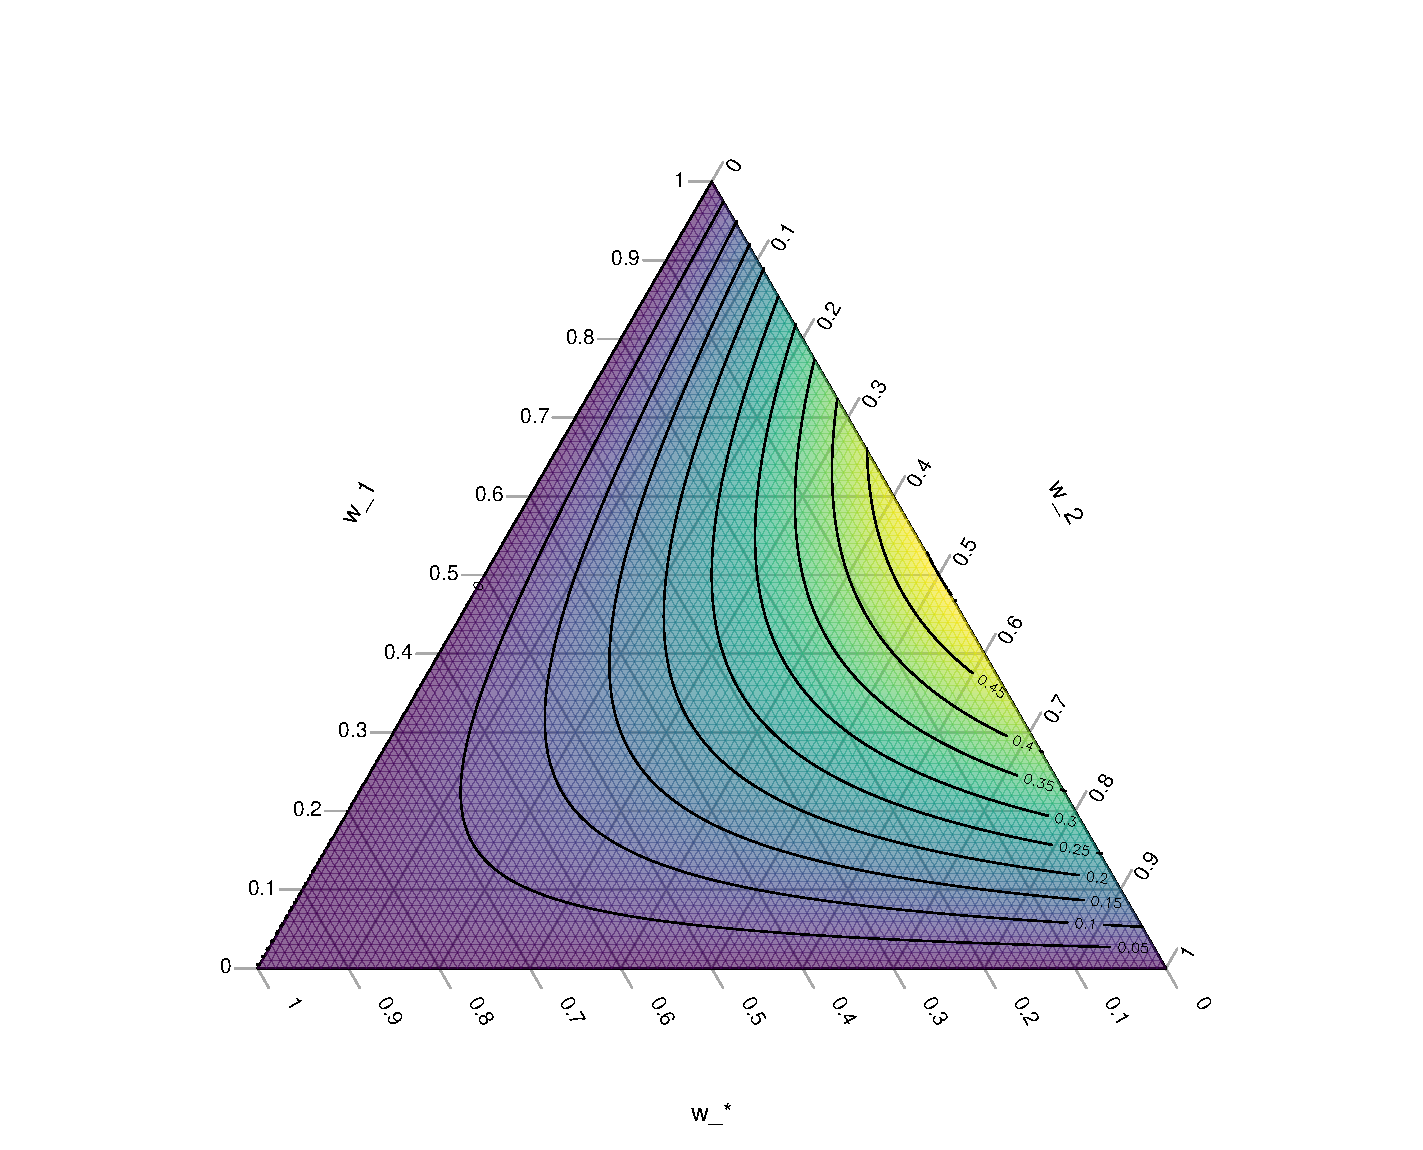
\includegraphics[width=0.7\textwidth]{ternplot1.pdf}
\caption{Plot of objective function $f(\mathbf{w})$ in the case $N=3$, where the immortal index is $i^*=3$.}
\label{fig:CSMC_ternaryplot}
\end{figure}


\begin{thm}
In conditional SMC with multinomial resampling, there exists $N_0$ such that for all $N>N_0$, for all finite $t$, $\PR[\tau_N(t) = \infty] =0$.
\end{thm}

%\begin{proof}
%As before, consider the sequence of events 
%$E_r := \{ c_N(r) > 2/N^2 \}$ for $r \in \mathbb{N}$.
%We know from the argument behind Lemma \ref{thm:nontrivial_csmc_optimalw} (which is completely analogous to Lemma \ref{thm:nontrivial_mn_optimalw}) that, in the case $\mathbf{w}=\mathbf{w}^*$, $E_r$ occurs infinitely often. Lemma \ref{lem:csmc_optimal_w} tells us that 
%$\PR[E_r \mid \mathbf{w}=(w_1, \dots, w_N)] \geq \PR[E_r \mid \mathbf{w}=\mathbf{w}^*]$
%for all $r$. 
%Therefore, by a coupling argument, we conclude that $E_r$ occurs infinitely often in the general case as well.
%\end{proof}

\begin{proof}
Combining Lemmata [4] and [6], we see that $\PR \left[c_N(t) > \frac{2}{N^2} \middle| \mathcal{H}_t \right] \geq 1- (\varepsilon(N-1))^{1-N} \prod_{i\neq i^*}^N h(X_{t-1}^{(i)})$ for all $t$. For sufficiently large $N$, say $N>N_0$, this probability is bounded away from zero.
[A D-separation + Borel--Cantelli argument analogous to the stochastic rounding case will lead to the result.]
\end{proof}

\subsection*{There's an easier way...}

\begin{thm}
In conditional SMC with multinomial resampling, there exists $N_0$ such that for all $N>N_0$, for all finite $t$, $\PR[\tau_N(t) = \infty] =0$.
\end{thm}

\begin{proof}
We have, from the proof of Corollary 2 in the draft paper,
\begin{equation*}
\E [c_N(t) \mid \mathcal{F}_{t-1}] \geq \frac{1}{(N)_2} \left\{ \frac{2\varepsilon^2}{a^2} + \frac{(N)_3 \varepsilon^4}{(N-1)^2 a^4} \right\} .
\end{equation*}
Since $c_N(t) \in [0,1]$ almost surely, for any fixed $N$ the ``worst-case'' distribution of $c_N(t)$ (i.e.\ maximising $\PR[c_N(t)=0 \mid \mathcal{F}_{t-1}]$) is two atoms, at 0 and 1. To ensure the correct expectation, the atom at 1 must have weight $\E[c_N(t) \mid \mathcal{F}_{t-1}]$, which is bounded below by the above inequality.
Hence for any finite $N$,
\begin{equation*}
\sum_{t=0}^\infty \PR[ c_N(t) > 2/N^2 \mid \mathcal{F}_{t-1}] 
\geq \sum_{t=0}^\infty \frac{1}{(N)_2} \left\{ \frac{2\varepsilon^2}{a^2} + \frac{(N)_3 \varepsilon^4}{(N-1)^2 a^4} \right\}
= \infty .
\end{equation*}
By Borel--Cantelli, we therefore have almost surely for all $N>2$ that $c_N(t) > 2/N^2$ for infinitely many $t$, which as argued earlier implies $\PR[\tau_N(t) = \infty] =0$ for all finite $t$.
\end{proof}


\section*{Stochastic rounding}
\begin{lemma} \label{lem:extreme_w_coal_as}
Let $\mathbf{w} = (w_1,\dots,w_N) \in \mathcal{S}_{N-1}$ and resample by stochastic rounding.
\begin{enumerate}[label=(\roman*)]
\item If $w_i \geq 2/N$ for some $i$, then $\PR[c_N(t) =0 |\mathbf{w} ] =0$. \label{item:SR_weight_2}
\item If $w_i= 0$ for some $i$, then $\PR[c_N(t) =0 |\mathbf{w} ] =0$. \label{item:SR_weight_0}
\end{enumerate}
\end{lemma}

\begin{proof}
In case \ref{item:SR_weight_2} particle $i$ is assigned at least two offspring, so $c_N(t)$ cannot be equal to zero.
In case \ref{item:SR_weight_0} particle $i$ is assigned zero offspring, so at least one other particle must be assigned more than one offspring, thus $c_N(t)$ cannot be equal to zero.
\end{proof}

The upshot of Lemma \ref{lem:extreme_w_coal_as} is that in these cases of ``extreme weights'' we have $c_N(t) > 2/N^2$ almost surely, so we can exclude these cases while we go about bounding $\PR[c_N(t) > 2/N^2 | \mathbf{w}]$ away from zero.


\begin{lemma}\label{lem:weps_cN_prob}
Define $\mathbf{w}^\delta := \frac{1}{N}\{(1,\dots,1) + \delta \mathbf{e}_i - \delta \mathbf{e}_j \}$ for any $i \neq j$ and $0< \delta < 1$. Then $\PR[c_N(t) > 2/N^2 | \mathcal{H}_t, \mathbf{w}_t = \mathbf{w}_\delta] \geq \delta \varepsilon^3$.
\end{lemma}

\begin{proof}
We use a bound on $\PR[ \nu_t^{(i)} = \lfloor N w_t^{(i)} \rfloor ]$ from the proof of Corollary 1 in the draft paper:
\begin{equation*}
\PR[ \nu_t^{(i)} = \lfloor N w_t^{(i)} \rfloor \mid \mathcal{H}_t] =: p_0 = 1-p_1 \leq 1 - (Nw_t^{(i)} - \lfloor N w_t^{(i)} \rfloor ) \varepsilon^{(2\lfloor N w_t^{(i)} \rfloor +1)} .
\end{equation*}
Then
\begin{align*}
\PR[c_N(t) \leq 2/N^2 | \mathcal{H}_t, \mathbf{w}_t = \mathbf{w}_\delta]
&= \PR[\nu_t^{(1:N)} = (1,\dots, 1) \mid \mathcal{H}_t, \mathbf{w}_t = \mathbf{w}_\delta] \\
&= \PR[\nu_t^{(i)} = 1, \nu_t^{(j)} = 1 \mid \mathcal{H}_t, \mathbf{w}_t = \mathbf{w}_\delta] \\
&= \PR[\nu_t^{(i)} = 1 \mid \mathcal{H}_t, \mathbf{w}_t = \mathbf{w}_\delta] \\
&\leq 1- (N w_\delta^{(i)} - \lfloor N w_\delta^{(i)} \rfloor) \varepsilon^{(2\lfloor N w_\delta^{(i)} \rfloor +1)} \\
&= 1- \{N(1+ \delta)/N - 1\}\varepsilon^3 \\
&= 1 - \delta\varepsilon^3 ,
\end{align*}
since the offspring counts are deterministically equal to one apart from particles $i$ and $j$, and it remains that $\nu_t^{(i)} = 1$ if and only if $\nu_t^{(j)} = 1$.
\end{proof}




\begin{lemma}
For any $\delta \in (0, 1)$, denote $\mathcal{S}_{N-1}^\delta := \{ \mathbf{w} \in \mathcal{S}_{N-1} :  \forall i, \, 0 <w_i <\frac{2}{N} ;\, \max_i w_i \geq \frac{1 + \delta}{N} \}$.
Then for all $\mathbf{w} \in \mathcal{S}_{N-1}^\delta$, 
$\PR[c_N(t) > 2/N^2 | \mathbf{w} ] \geq \PR[c_N(t) > 2/N^2 | \mathbf{w}_\delta ]$.
\end{lemma}

\begin{proof}
Fix arbitrary $\mathbf{w} \in \mathcal{S}_{N-1}^\delta$. Let $i^*$ be then index of the particle with the largest weight.
Denote $\mathcal{I} := \{i \in \{1,\dots,N\} : w_i > 1/N \}$.
Notice that 
\begin{equation*}
\PR[ c_N(t) \leq 2/N^2 | \mathbf{w} ] 
= \PR[ \nu_t^{(i)} =1 \,\forall i\in\{1,\dots,N\} | \mathbf{w}] 
= \PR[ \nu_t^{(i)} =1 \,\forall i\in \mathcal{I} | \mathbf{w}] .
\end{equation*}
This is true because all weights are in $(0, 2/N)$, so for $i \in \mathcal{I}, \nu_t^{(i)} \in \{1,2\}$, and for $i \notin \mathcal{I}, \nu_t^{(i)} \in \{0,1\}$; and the offspring counts must sum to $N$ (a generalisation of the argument used in Lemma \ref{lem:weps_cN_prob}).

We can then decompose this probability into a product of conditional probabilities:
\begin{align*}
\PR[ \nu_t^{(i)} =1 \,\forall i\in \mathcal{I} | \mathbf{w}]
&= \prod_{i \in \mathcal{I}} \PR[ \nu_t^{(i)} =1 | \nu_t^{(j)}=1 \,\forall j <i \in \mathcal{I}; \mathbf{w}] \\
&= \PR[\nu_t^{(i^*)} =1 | \mathbf{w}] \prod_{i \neq i^* \in \mathcal{I}} \PR[ \nu_t^{(i)} =1 | \nu_t^{(i^*)}=1; \nu_t^{(j)}=1 \,\forall j <i \in \mathcal{I}; \mathbf{w}] \\
&\leq \PR[\nu_t^{(i^*)} =1 | \mathbf{w}] .
\end{align*}
The last line is equal to the probability $\PR[ c_N(t) \leq 2/N^2 | \mathbf{w} ] $ in the case where $|\mathcal{I}| =1$, i.e.\ the only weight larger than $1/N$ is $w_{i^*}$.

In other words, $\PR[ c_N(t) > 2/N^2 | \mathbf{w} ]$ is minimised on $\mathcal{S}_{N-1}^\delta$ by having only one weight larger than $1/N$, in which case the values of the other weights do not affect this probability. 

We therefore find that a minimum of $\PR[ c_N(t) > 2/N^2 | \mathbf{w} ]$ on $\mathcal{S}_{N-1}^\delta$ is given by $\mathbf{w}_{\delta^\prime}$, for some $\delta^\prime \geq \delta$. 
It only remains to show that taking $\delta^\prime > \delta$ does not decrease the probability. This is a consequence of Lemma \ref{lem:weps_cN_prob}, where we see that $\PR[ c_N(t) > 2/N^2 | \mathbf{w}_{\delta^\prime}]$ is monotonically increasing in $\delta^\prime$.
Thus the minimum of $\PR[ c_N(t) > 2/N^2 | \mathbf{w} ]$ is attained at $\mathbf{w} = \mathbf{w}_\delta$, as required. (Although this minimum is not unique, we have shown explicitly that it is a global minimum on $\mathcal{S}_{N-1}^\delta$.)
\end{proof}

\begin{thm}
Consider a sequential Monte Carlo algorithm using any stochastic rounding as its resampling scheme.
If there exists $\mu>0$ such that $\PR\{\max_i w_t^{(i)} \geq (1+\delta)/N \mid \mathcal{H}_t\} \geq \mu$ for infinitely many $t$ then $\PR\{\tau_N(t) = \infty \}=0$ for all $N>1$ and for all finite $t$.
\end{thm}

\begin{proof}
Combining Lemmata [7--9] we see that, for any $\mathbf{w} \in \mathcal{S}_{N-1}$ such that $\max_i w_i \geq \frac{1 + \delta}{N}$, we have the bound $\PR[ c_N(t) > 2/N^2 | \mathbf{w} ] \geq \delta\varepsilon^3$.
By the law of total probability,
\begin{equation*}
\PR[c_N(t) > 2/N^2 \mid \mathcal{H}_t] 
\geq \PR[c_N(t) > 2/N^2 \mid \mathcal{H}_t, \max w_i \geq (1+\delta)/N ]\, \PR[\max w_i \geq (1+\delta)/N \mid \mathcal{H}_t]
\geq \mu \delta \varepsilon^3 
\end{equation*}
for those infinitely many $t$ where $\PR\{\max_i w_t^{(i)} \geq (1+\delta)/N \mid \mathcal{H}_t\} \geq \mu$.
Using the D-separation established in [draft paper, Cor 1 proof], we can write
\begin{align*}
\PR[c_N(t) > 2/N^2 \mid \mathcal{F}_{t-1}] 
&= \E[ \I{c_N(t) > 2/N^2} \mid \mathcal{F}_{t-1}] \\
&= \E[ \E[ \I{c_N(t) > 2/N^2} \mid \mathcal{H}_t ]\mid \mathcal{F}_{t-1}] \\
&= \E[ \PR[c_N(t) > 2/N^2 \mid \mathcal{H}_t ]\mid \mathcal{F}_{t-1}] .
\end{align*}
Hence this probability is bounded below by $\mu\delta\varepsilon^3$ for infinitely many $t$. We therefore have
\begin{equation}
\sum_{t=0}^\infty \PR[c_N(t) > 2/N^2 \mid \mathcal{F}_{t-1}]  \geq \sum_{j=0}^\infty \mu\delta\varepsilon^3 = \infty ,
\end{equation}
and applying Theorem [1 - that BC2 statement], almost surely $c_N(t) >2/N^2$ for infinitely many $t$.
As argued in Lemma [2], this is sufficient for the result.
\end{proof}


\end{document}